%TC第29.1节练习 4、5
%TC第29.2节练习 2、4、6
%TC第29.3节练习 5
%TC第29.4节练习 2
%%%%%%%%%%%%%%%%%%%%%%%%%%%%%%%%%%%%%%%%%%%%%%%%%%%%%%%%%%%%%%%%
\documentclass[11pt, a4paper, UTF8]{ctexart}
%%%%%%%%%%%%%%%%%%%%%%%%%%%%%%%%%%%
% File: preamble.tex
%%%%%%%%%%%%%%%%%%%%%%%%%%%%%%%%%%%

\usepackage[top = 1.5cm]{geometry}

% Set fonts commands
\newcommand{\song}{\CJKfamily{song}} 
\newcommand{\hei}{\CJKfamily{hei}} 
\newcommand{\kai}{\CJKfamily{kai}} 
\newcommand{\fs}{\CJKfamily{fs}}

\newcommand{\me}[2]{\author{{\bfseries 姓名:}\underline{#1}\hspace{2em}{\bfseries 学号:}\underline{#2}}}

% Always keep this.
\newcommand{\noplagiarism}{
  \begin{center}
    \fbox{\begin{tabular}{@{}c@{}}
      请独立完成作业,不得抄袭。\\
      若得到他人帮助, 请致谢。\\
      若参考了其它资料,请给出引用。\\
      鼓励讨论,但需独立书写解题过程。
    \end{tabular}}
  \end{center}
}

% Each hw consists of three parts:
% (1) this homework
\newcommand{\beginthishw}{\part{作业}}
% (2) corrections (Optional)
\newcommand{\begincorrection}{\part{订正}}
% (3) any feedback (Optional)
\newcommand{\beginfb}{\part{反馈}}

% For math
\usepackage{amsmath}
\usepackage{amsfonts}
\usepackage{amssymb}

% Define theorem-like environments
\usepackage[amsmath, thmmarks]{ntheorem}

\theoremstyle{break}
\theorembodyfont{\song}
\theoremseparator{}
\newtheorem*{problem}{题目}


\theoremheaderfont{\kai\bfseries}
\theoremseparator{:}
% \newtheorem*{remark}{注}
\theorempostwork{\bigskip\hrule}
\newtheorem*{solution}{解答}
\theorempostwork{\bigskip\hrule}
\newtheorem*{revision}{订正}

\theoremstyle{plain}
\newtheorem*{cause}{错因分析}
\newtheorem*{remark}{注}

\theoremstyle{break}
\theorempostwork{\bigskip\hrule}
\theoremsymbol{\ensuremath{\Box}}
\newtheorem*{proof}{证明}

\renewcommand\figurename{图}
\renewcommand\tablename{表}

% For figures
% for fig with caption: #1: width/size; #2: fig file; #3: fig caption
\newcommand{\fig}[3]{
  \begin{figure}[htp]
    \centering
      \includegraphics[#1]{#2}
      \caption{#3}
  \end{figure}
}

% for fig without caption: #1: width/size; #2: fig file
\newcommand{\fignocaption}[2]{
  \begin{figure}[htp]
    \centering
    \includegraphics[#1]{#2}
  \end{figure}
}

\title{4-1:线性规划 [课前]}
\me{张天昀}{171860508}
\date{\today}

\begin{document}
\maketitle
\noplagiarism

%%%%%%%%%%%%%%%%%%%%%%%%%%%%%%%%%%%%%%%%%%%%%%%%%%%%%%%%%%%%%%%%
%                       Homework START!                        %
%%%%%%%%%%%%%%%%%%%%%%%%%%%%%%%%%%%%%%%%%%%%%%%%%%%%%%%%%%%%%%%%
\beginthishw
%%%%%%%%%%%%%%%%%%%%
\begin{problem}[TC 29.1-4]
Convert the following linear program into standard form:\\
minimize
\begin{center}
\begin{tabular}{r r r r r r r}
$2x_1$& $+$ & $7x_2$ & $+$ & $x_3$ & & 
\end{tabular}
\end{center}
subject to
\begin{center}
\begin{tabular}{r r r r r r r}
$x_1$ & & & $-$ & $x_3$ & $=$ & 7\\
$3x_1$ & + & $x_2$ & & & $\geqslant$ & 24\\
 & & $x_2$ & & & $\geqslant$ & 0 \\
 & & & & $x_3$ & $\leqslant$ & 0 \\
\end{tabular}
\end{center}
\end{problem}
\begin{solution}
    
\end{solution}




\begin{problem}[TC 29.2-2]
Write out explicitly the linear program corresponding to finding the shortest path from node $s$ to node $y$ in Figure 24.2(a).
\begin{center}
    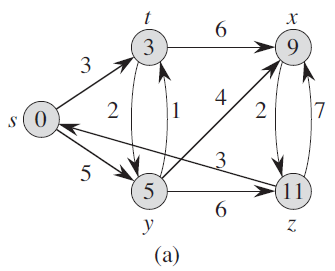
\includegraphics[scale=0.5]{24-2-a.png}
\end{center}
\end{problem}
\begin{solution}
    
\end{solution}




\begin{problem}[TC 29.2-4]
    Write out explicitly the linear program corresponding to finding the maximum flow
    in Figure 26.1(a).
\end{problem}
\begin{center}
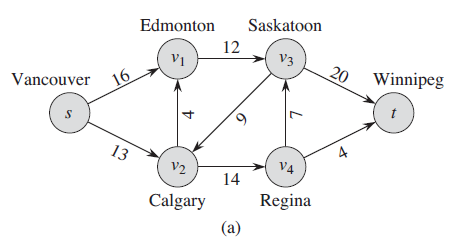
\includegraphics[scale=0.5]{26-1-a.png}
\end{center}
\begin{solution}
    
\end{solution}




\begin{problem}[TC 29.2-6]
Write a linear program that, given a bipartite graph $G =(V,E)$, solves the maximum-bipartite-matching problem.
\end{problem}
\begin{solution}
    
\end{solution}





\begin{problem}[TC 29.3-5]
Solve the following linear program using \textsc{Simplex}:
maximize 
\begin{center}
\begin{tabular}{rrrrr}
$18x_1$ & $+$ & $12.5x_2$
\end{tabular}
\end{center}
subject to
\begin{center}
\begin{tabular}{rrrrr}
$x_1$ & $+$ & $x_2$ & $\leqslant$ & $20$ \\
$x_1$ & $ $ & $ $ & $\leqslant$ & $12$ \\
$ $ & $ $ & $x_2$ & $\leqslant$ & $16$ \\
$x_1,$ & $ $ & $x_2$ & $\geqslant$ & $0$ \\
%$ $ & $ $ & $ $ & $ $ & $ $ \\
\end{tabular}
\end{center}
\end{problem}
\begin{solution}
    
\end{solution}





\begin{problem}[TC 29.4-2]
Suppose that we have a linear program that is not in standard form. We could produce the dual by first converting it to standard form, and then taking the dual. It would be more convenient, however, to be able to produce the dual directly. Explain how we can directly take the dual of an arbitrary linear program.
\end{problem}
\begin{solution}
    
\end{solution}
%%%%%%%%%%%%%%%%%%%%%%%%%%%%%%%%%%%%%%%%%%%%%%%%%%%%%%%%%%%%%%%%
%                      Correction START!                       %
%%%%%%%%%%%%%%%%%%%%%%%%%%%%%%%%%%%%%%%%%%%%%%%%%%%%%%%%%%%%%%%%
%\begincorrection
%%%%%%%%%%%%%%%%%%%%
%\begin{problem}[]

%\end{problem}

%\begin{cause}
%
%\end{cause}

%\begin{revision}

%\end{revision}
%%%%%%%%%%%%%%%%%%%%
%\newpage
%%%%%%%%%%%%%%%%%%%%





%%%%%%%%%%%%%%%%%%%%%%%%%%%%%%%%%%%%%%%%%%%%%%%%%%%%%%%%%%%%%%%%
%                       Feedback START!                        %
%%%%%%%%%%%%%%%%%%%%%%%%%%%%%%%%%%%%%%%%%%%%%%%%%%%%%%%%%%%%%%%%
%\beginfb
%\begin{itemize}
%
%\end{itemize}





%%%%%%%%%%%%%%%%%%%%%%%%%%%%%%%%%%%%%%%%%%%%%%%%%%%%%%%%%%%%%%%%
%                        Homework END!                         %
%%%%%%%%%%%%%%%%%%%%%%%%%%%%%%%%%%%%%%%%%%%%%%%%%%%%%%%%%%%%%%%%
\end{document}
